\documentclass[9pt]{article}
\usepackage[colorlinks=true, allcolors=black]{hyperref}
\usepackage[table,xcdraw]{xcolor}
\usepackage[utf8]{inputenc}
\usepackage{graphicx}
\usepackage[colorinlistoftodos]{todonotes}
\usepackage[colorlinks=true, allcolors=black]{hyperref}
\usepackage{multirow}
\usepackage[spanish]{babel}
\selectlanguage{spanish}
% Esto es para poder escribir acentos directamente:
\usepackage[utf8]{inputenc}
\usepackage[T1]{fontenc}
\usepackage{enumitem}
\usepackage{movie15}
\usepackage{booktabs}
\usepackage{amssymb}
\usepackage{pifont}
\usepackage{tikz}
\usepackage[latin1]{inputenc}
%% Asigna un tamaño a la hoja y los márgenes
\usepackage[a4paper,top=1.65cm,bottom=1.65cm,left=2cm,right=2cm,marginparwidth=1.75cm]{geometry}
\usepackage{wrapfig}
\usepackage{fancyhdr}
\usepackage{multirow}
\usepackage{caption}
\usepackage{longtable}
\usepackage{gensymb}
\usepackage{float}
\usepackage[position=top]{subfig}
\usepackage{verbatim}
\setlength\parindent{7pt}
\setlength{\parskip}{3pt}
%% spce line 
\usepackage{setspace}
	\setstretch{1.1}
\usepackage{pdfpages}
%% Paquetes de la AMS
\usepackage{amsmath, amsthm, amsfonts}
\usepackage{tikz}
\usetikzlibrary{shapes.geometric}
\usetikzlibrary{shapes.arrows}
\usepackage{array} 
\usepackage[dvipsnames]{xcolor}
\usepackage{xcolor}
\usepackage{soul}
\newcommand{\mathcolorbox}[2]{\colorbox{#1}{$\displaystyle #2$}}
\date{}

\usepackage{apacite}
\bibliographystyle{apacite}
\usepackage[citestyle=authoryear,
    bibstyle=numeric,mergedate=false,sorting=ynt]{biblatex}
\assignrefcontextentries[]{*}
\renewbibmacro*{publisher+location+date}{%
  \printlist{publisher}%
  \setunit*{\addsemicolon\space}%
  \printlist{location}%
  \setunit*{\addsemicolon\space}%
  \usebibmacro{date}%
  \newunit%
}
\addbibresource{bibliografia.bib}


\begin{document}

\begin{titlepage} % Suppresses displaying the page number on the title page and the subsequent page counts as page 1
	\newcommand{\HRule}{\rule{\linewidth}{0.5mm}} % Defines a new command for horizontal lines, change thickness here
	
	\center % Centre everything on the page
	
	%------------------------------------------------
	%	Headings
	%------------------------------------------------
	
\includegraphics[width=0.7\textwidth]{logoudesa.jpg}\\[0.8cm]
	
	\textsc{\LARGE Herramietas Computacionales para la Investigación}\\[0.5cm] % Major heading such as course name
	
	\textsc{\Large Amelia Gibbons}\\

	%------------------------------------------------
	%	Title
	%------------------------------------------------
	\textcolor{white}{\HRule}\\[0.6cm]
	\huge\bfseries Trabajo Final 
	\textcolor{white}{\HRule}\\[1.5cm]
	%------------------------------------------------
	%	Author(s)
	%------------------------------------------------
	\begin{center}
		\Large
		\textsc{Liwski, Sury}\\
	\end{center}
	
	% If you don't want a supervisor, uncomment the two lines below and comment the code above
	%{\large\textit{Author}}\\
	%John \textsc{Smith} % Your name
	
	%------------------------------------------------
	%	Date
	%------------------------------------------------
	\vfill\vfill\vfill % Position the date 3/4 down the remaining page
	{\large 2022}
	\vfill
	
\end{titlepage}
\section*{Introducci\'on}
La consigna de este trabajo final consiste en usar los datos georeferenciados de algún paper y generar mapas y gráficos que puedan ayudar a los resultados/conclusiones del paper, as\'i como presentar de otra manera los datos. Para dar respuesta, elegimos y utilizamos \cite{10.1257/pol.6.4.71}. 

Si bien este no est\’a georreferenciado, como explayaremos a continuaci\’on, dado que presenta datos abiertos a nivel municipio de much\’isimas variables para M\’exico por un largo per\’iodo de tiempo bien codificados, de combinarlo con el \texttt{.shp} publicado por~\cite{shapefile}, se pueden georeferenciar todos estos datos \texttt{.do}

Explotamos que su estrategia de identificaci\'on es \textit{DiD - Event Studies} con observaciones a nivel municipio y los datos que ello conlleva para realizar gr\'aficos a tanto est\'aticos a nivel municipio, como de la evoluci\'on de ciertas variables en el tiempo. Adem\'as, incluimos una animaci\'on que contempla ambos casos.

Adem\’as de varios archivos \texttt{.do} y sus respectivas figuras, los autores comparten entre sus datos varias carácter\’isticas demogr\’aficas y geogr\’aficas a nivel municipio provistas por el XII Censo General de Población y Vivienda 2000 de M\’exico; empleados y empleadores adheridos al IMSS durante varios a\~nos a nivel municipio;  la cantidad de familias e individuos afiliados al Seguro Popular durante varios a\~nos por municipio; datos de pobreza por municipio para los a\~nos 2000 y 2005; gobernantes por a\~no; afiliados a otros seguros por a\~no; municipios encontrados en la ENOE; y un dataset para poder combinar todo esto.

Con ello, realizamos el siguiente trabajo. Se hace entrega de los siguientes gr\’aficos, exportados como \textt{.eps} de dimensiones justas para este tama\~no de p\’agina, con la intenci\’on de poder poner dos gr\’aficos por p\’agina y una breve descripci\’on del mismo.\textbf{ La extensi\'on con la cual se incluyen los gr\'aficos nos permiten hacer zoom a los mapas en el pdf y que se vean bien el detalle de los l\'imites, resolviendo el problema de congesti\'on de municipios al centro sur del pa\'is si son mapas. Es cuesti\'on de hacer zoom para diferenciar bien, dado que los datos son a nivel municipio, habiendo algunos peque\~nos relativo al tama\~no de M\'exico.} Varios son nuevos, pero hay algunas figuras replicadas del paper. Estas \’ultimas son solamente con la intenci\’on de demostrar que podemos replicar un gr\’afico realizado en \texttt{STATA} en \texttt{R}, ya que como mencionamos antes, todos los códigos de los autores son de acceso p\’ublico. Adem\’as, \textbf{se hace entrega de un GIF que muestra como los municipios van entrando al programa a lo largo del tiempo}, considerando entrada de un municipio al programa de la misma manera que en el paper\footnote{M\’as de diez individuos en un municipio adheridos al Seguro Popular.}. 

Todos los archivos, datos y c\’odigos pueden ser encontrados en el correspondiente repositorio de \href{https://github.com/joaquinliwski/Herramientas-Computacionales-Liwski-Sury-Trabajo-Final.git}{GitHub}. Cabe aclarar que, a diferencia de lo tratado en el curso, se utilizara el paquete de \texttt{R} llamado \texttt{SF}. Esto implica una mejor estructura de los datos, \textit{simple features}, estando en una sola fila toda la geometr\'ia de un dicha observaci\'on. No utilizaremos las funciones \texttt{geom\_polygon()} y similares, sino que las reemplazaremos por \texttt{geom\_sf()} y similares. 
La intenci\'on con este trabajo es presentar parte de la informaci\'on de otras maneras. Especialmente lo que corresponde a cada municipio. 

\section*{Resumen del Trabajo}
\cite{10.1257/pol.6.4.71}  analizan el efecto del programa Seguro Popular (SP) en el mercado laboral mexicano. Los autores argumentan que al proveer seguro medico gratuito a los trabajadores informales, alteró los incentivos de operar en el mercado formal. Especificamente, encuentran que el SP tuvo un efecto negativo en el número de empleadores y empleados registrados formalmente en las firmas chicas y medianas (hasta 50 empleados). Según sus estimaciones, en ausencia del SP entre 2000 y 2011, 36,000 empleadores y 171,000 empleados adicionales deberían haberse registrado en el Instituto Mexicano de Seguridad Social (IMSS) en empresas con menos de 50 empleados. De este modo, las ganancias del acceso a cobertura medica, vinculadas principalmente a la reducción de gastos catastróficos en salud, deben ponderarse en contra de las implicancias de esta reasignación del trabajo fuera de la formalidad. Se destacan tres efectos negativos sobre el bienestar de esta reasignación: pérdida de ingresos tributarios, pérdida de beneficios adicionales de formalidad para los trabajadores y pérdidas de productividad.

\section*{Replicando Figuras}
 Como mencionamos previamente, esto es solamente con la intenci\'on de demostrar que lo podemos replicar en otro software. Todos los c\'odigos originales del trabajo son de acceso p\'ublico.
 
 A continuaci\'on se replica la Figura 1 del trabajo, en la cu\'al los autores retratan en dos ejes distintos la evoluci\'on de empleados y empleadores asociados al Seguro Social Mexicano.
 \begin{figure}[H]
     \centering
     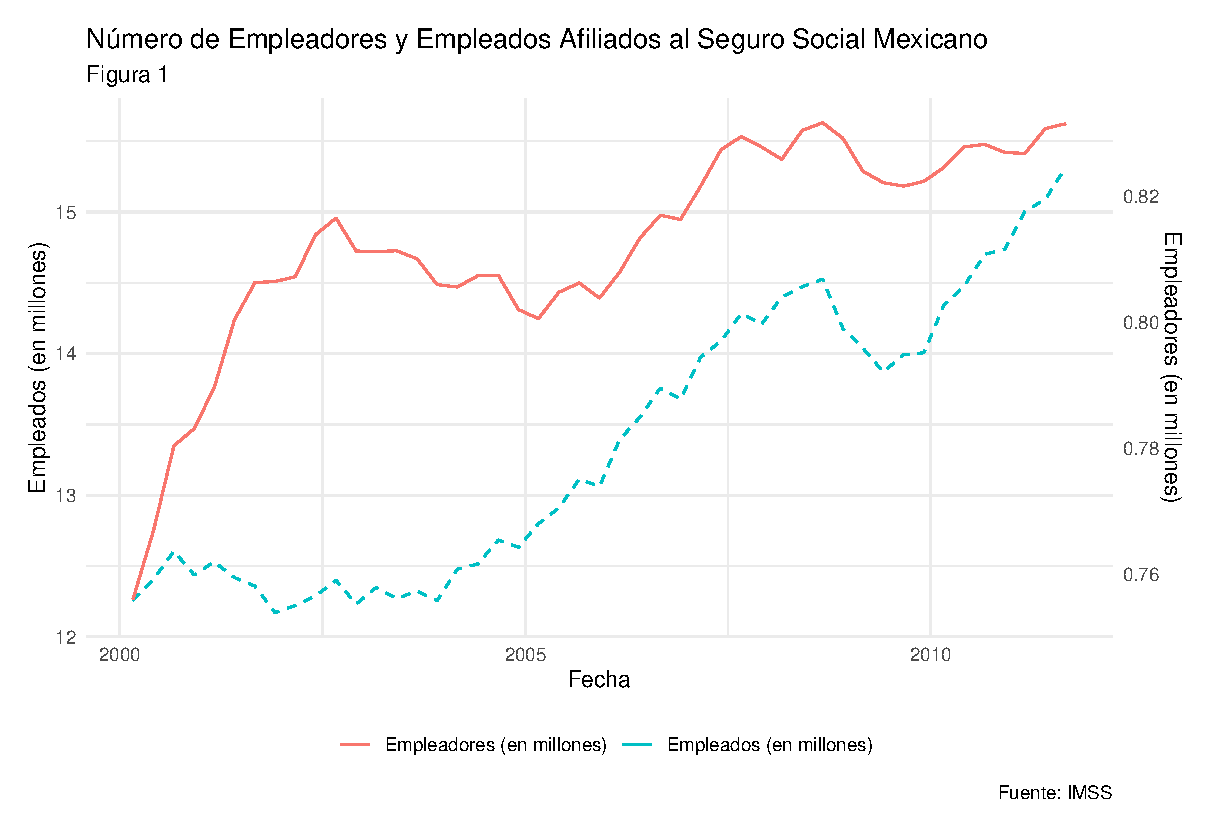
\includegraphics[width=0.95\textwidth]{figs/employement.eps}
     \label{fig1}
 \end{figure}
 Luego, en la siguiente figura, replicamos la Figura 3. En esta, los autores muestran la evoluci\'on de afiliados a distintos programas de seguro m\'edico.
  \begin{figure}[H]
     \centering
     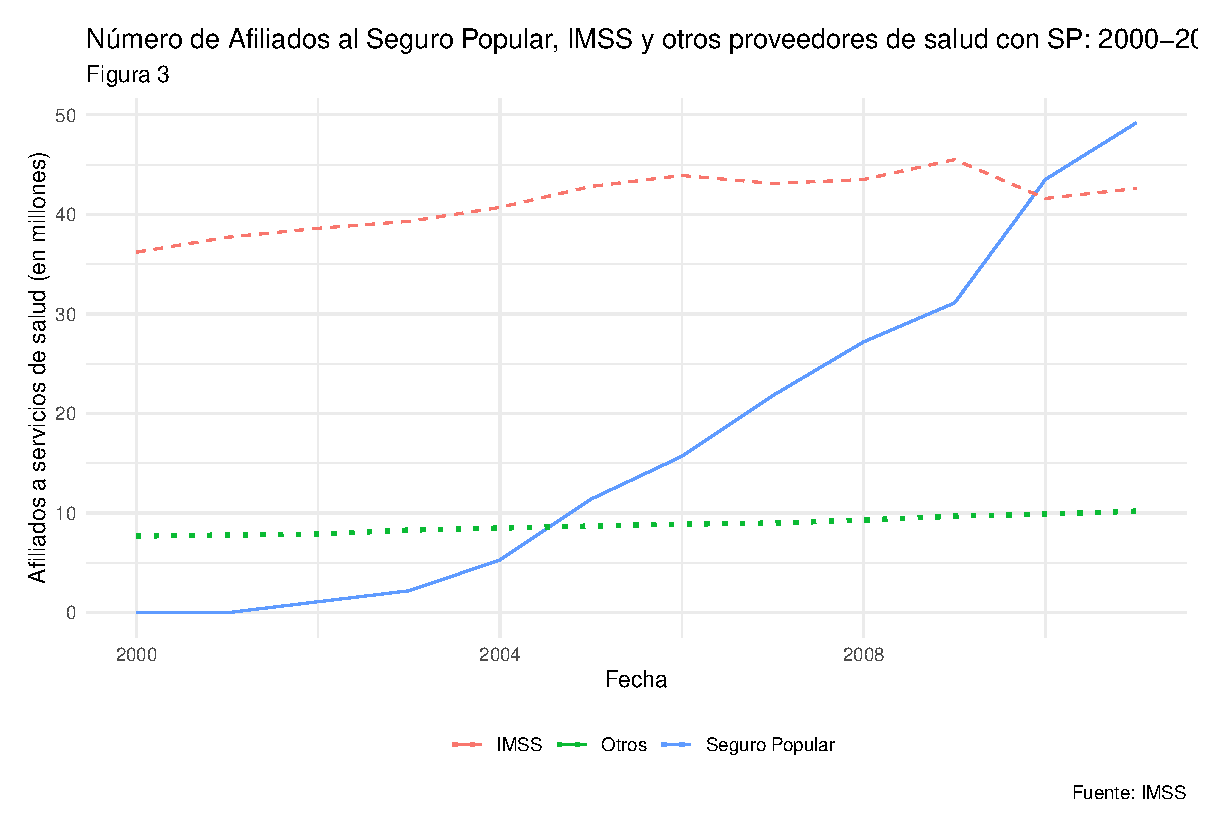
\includegraphics[width=0.95\textwidth]{figs/figura3.eps}
     \label{fig3}
 \end{figure}
 \section*{Caracter\'isticas por Municipio}
 Utilizando los datos compartidos por los autores obtenidos del XII Censo General de Población y Vivienda 2000 de M\'exico, presentamos varios mapas y gr\'aficos a modo descriptivo.
 
 En lo que a pobreza respecta, presentamos los siguientes mapas con los porcentajes de pobreza tanto alimentaria como por ingresos. 
 
 \begin{figure}[H]
     \centering
     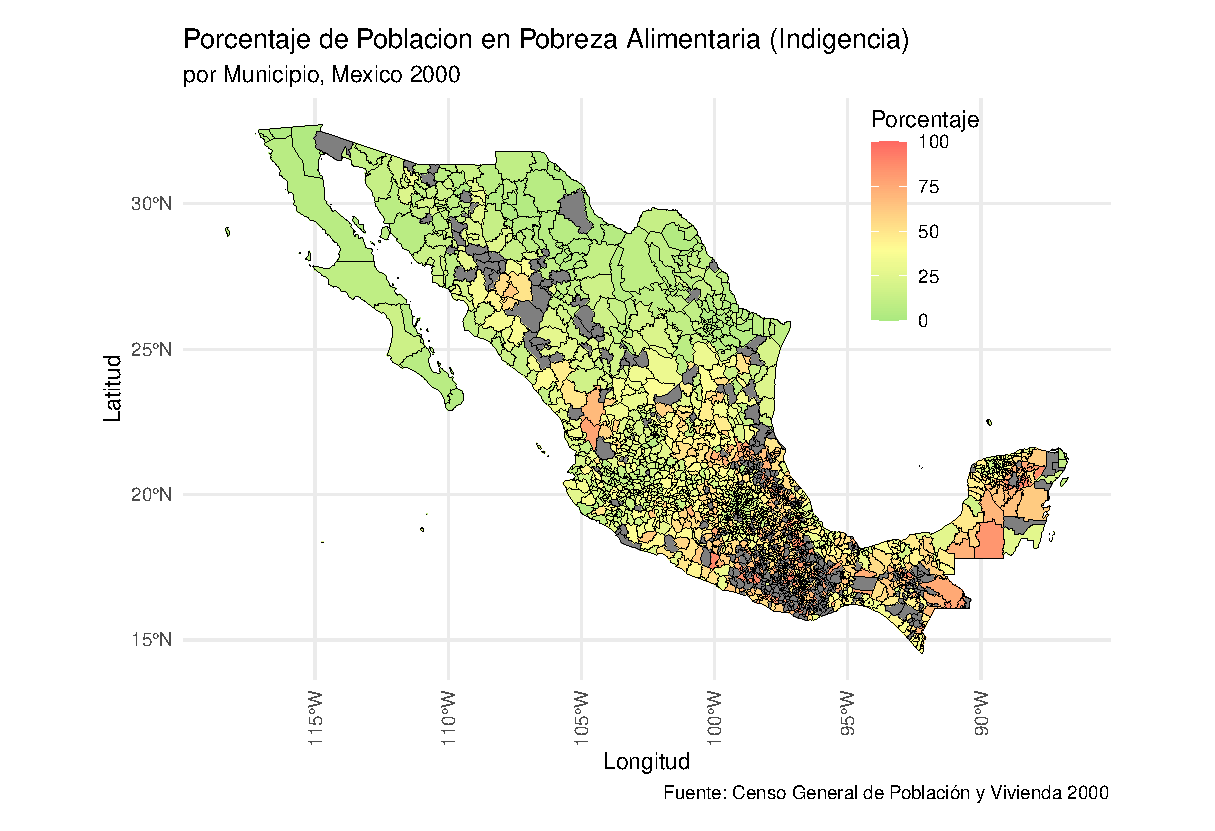
\includegraphics[width=0.97\textwidth]{figs/povertyalim.eps}
 \end{figure}
 
  \begin{figure}[H]
     \centering
     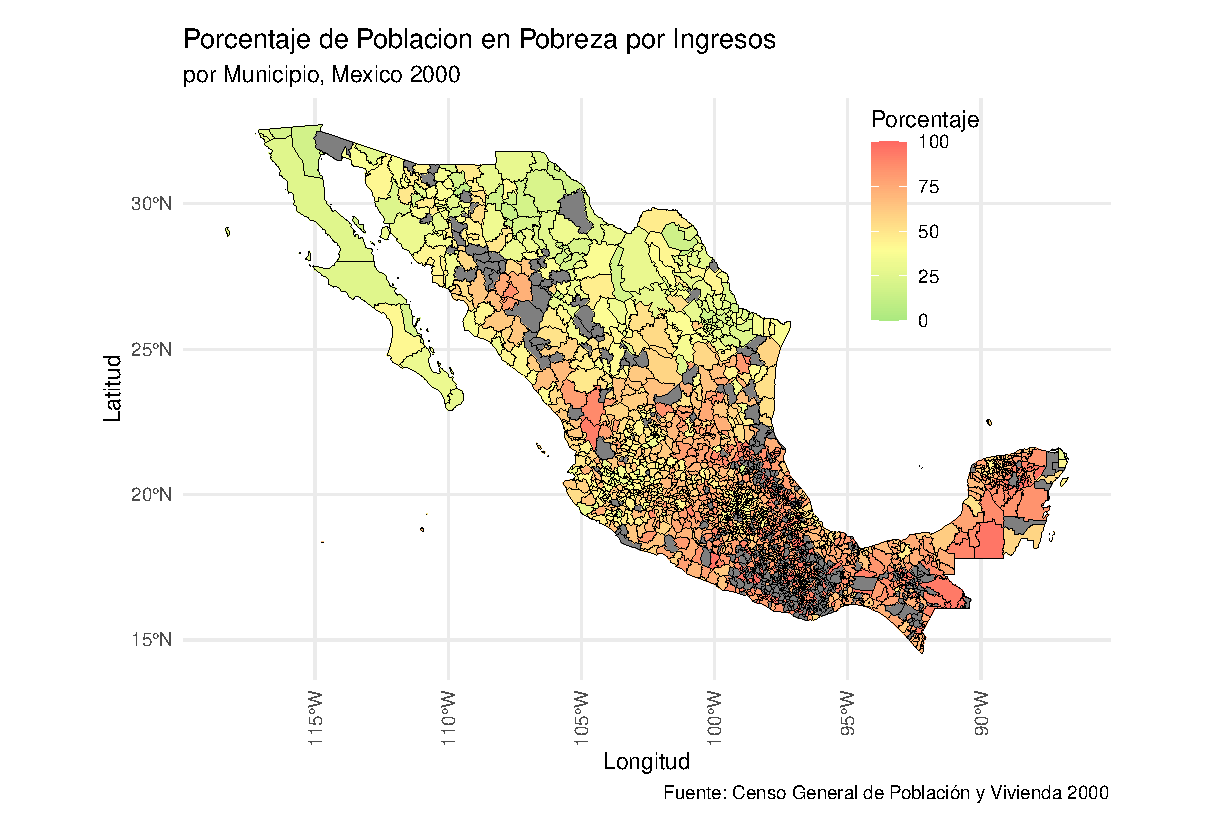
\includegraphics[width=0.97\textwidth]{figs/povertypat.eps}
 \end{figure}
 A continuaci\'on se grafica la poblaci\'on por municipio. Este es un ejemplo de un mal gr\'afico, ya que la misma no es robusta al tama\~no del municipio. Sumado a esto, la presencia de diversos valores extremos no permite diferenciar entre los municipios que presentan un nivel similar de poblaci\'on, resultando en un problema, dado que la mayor parte de la distribuci\'on de poblaci\'on en municipios se encuentra cercana a un mismo n\'umero. 
 
 Lo ideal ser\'ia graficar densidad poblacional, pero como no contamos con esos datospresentamos este como \textit{second best}, destacando cual es el error de hacer esto.  Lo dejamos de todos modos ya que de el GIF tmbi\'en considera cantidad total de individuos adheridos en la escala de colores. 
   \begin{figure}[H]
     \centering
     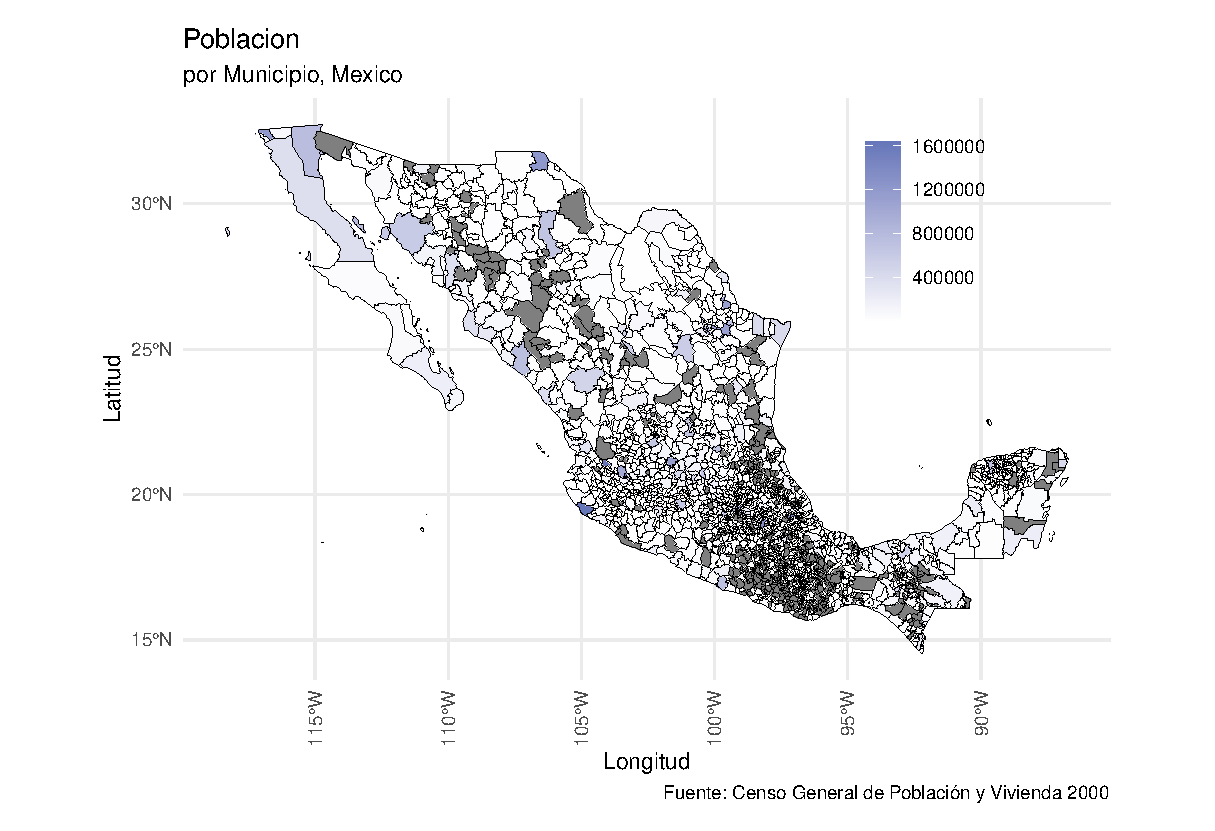
\includegraphics[width=0.9\textwidth]{figs/populationb.eps}
 \end{figure}
 A continuaci\'on, dividimos los municipios de M\'exico entre lo que los autores consideran urbanos y rurales. Se puede observar, de compararlo con el GIF, que por lo general se adhieren primero al programa los municipios urbanos. 
    \begin{figure}[H]
     \centering
     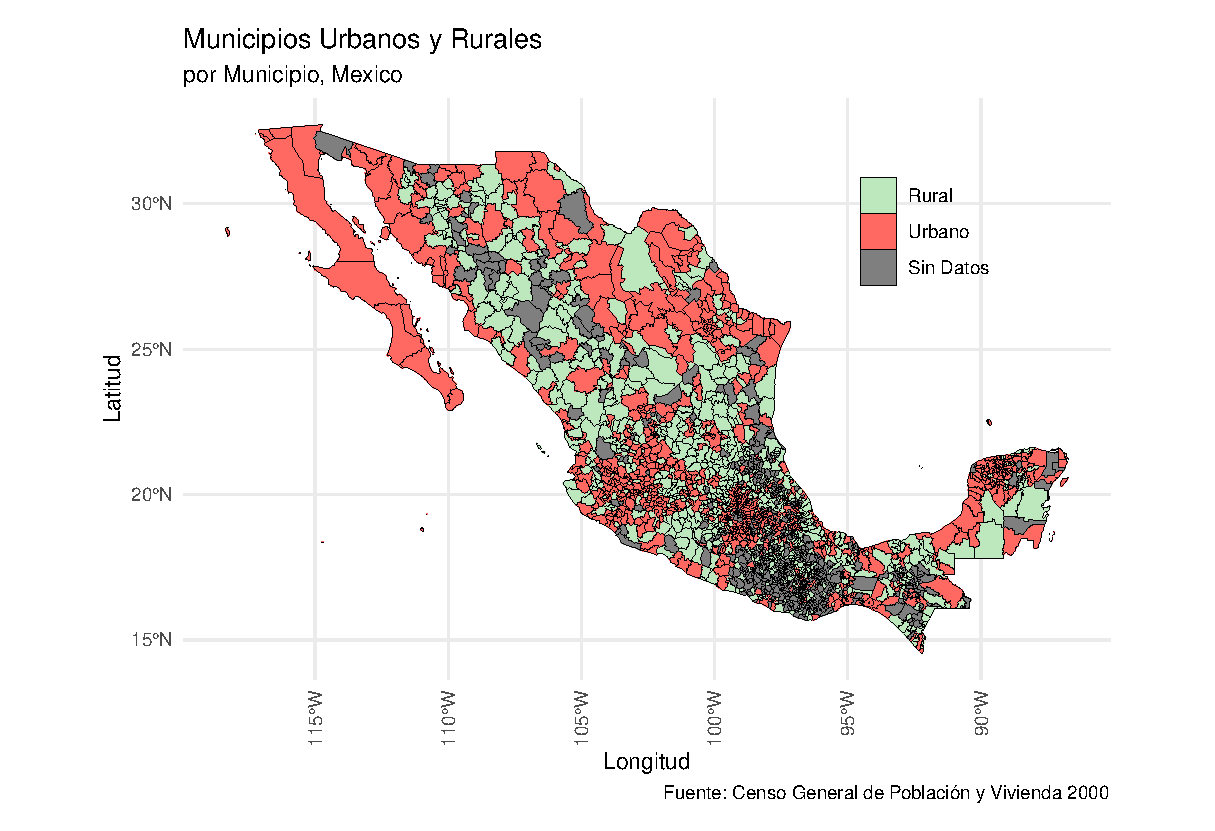
\includegraphics[width=0.9\textwidth]{figs/Urbanos y Rurales.eps}
 \end{figure}
\newpage Dado que el paper corresponde al impacto sobre distintas variables relacionadas al ámbito laboral, a continuación se presentan mapas con informalidad (entendida como quienes no aportan al IMSS). 

\begin{figure}[H]
     \centering
     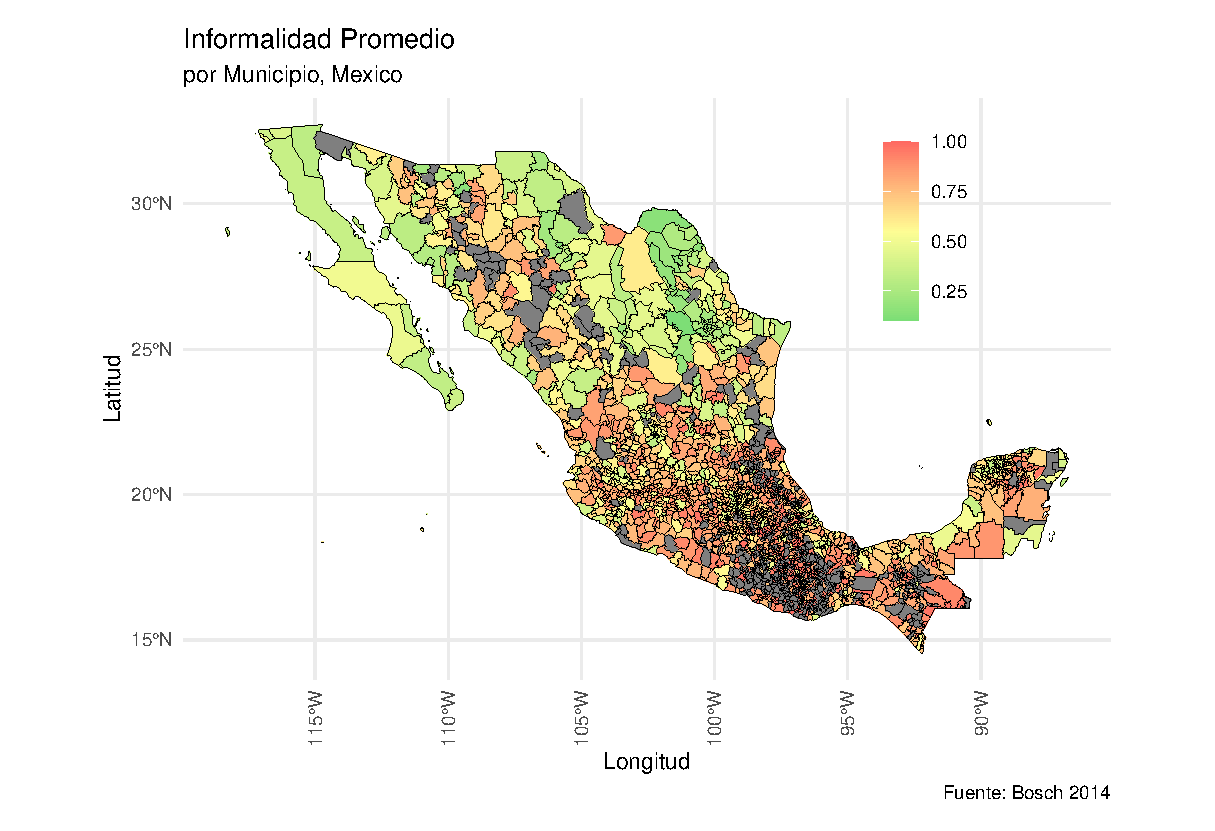
\includegraphics[width=\textwidth]{figs/inf.eps}
 \end{figure}

 A continuaci\'on se presenta la distribuci\'on de la informalidad.
 \begin{figure}[H]
     \centering
     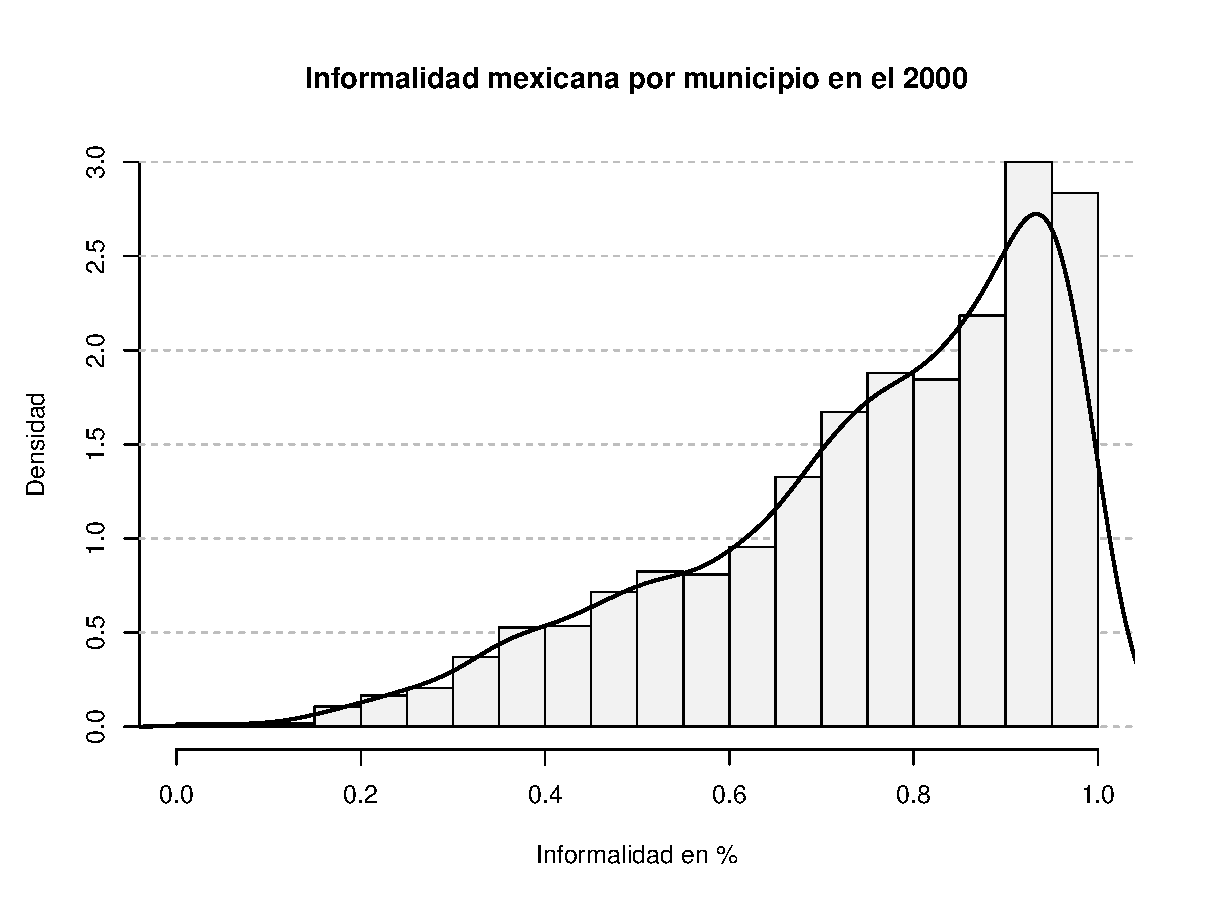
\includegraphics[width=0.8\textwidth]{figs/histinf.eps}
 \end{figure}
 \newpage
 Teniendo en cuenta los distintos seguros a los que se puede un empleado afiliar, se presenta el siguiente mapa de proporci\'on de poblaci\'on afiliada. 

\begin{figure}[H]
     \centering
     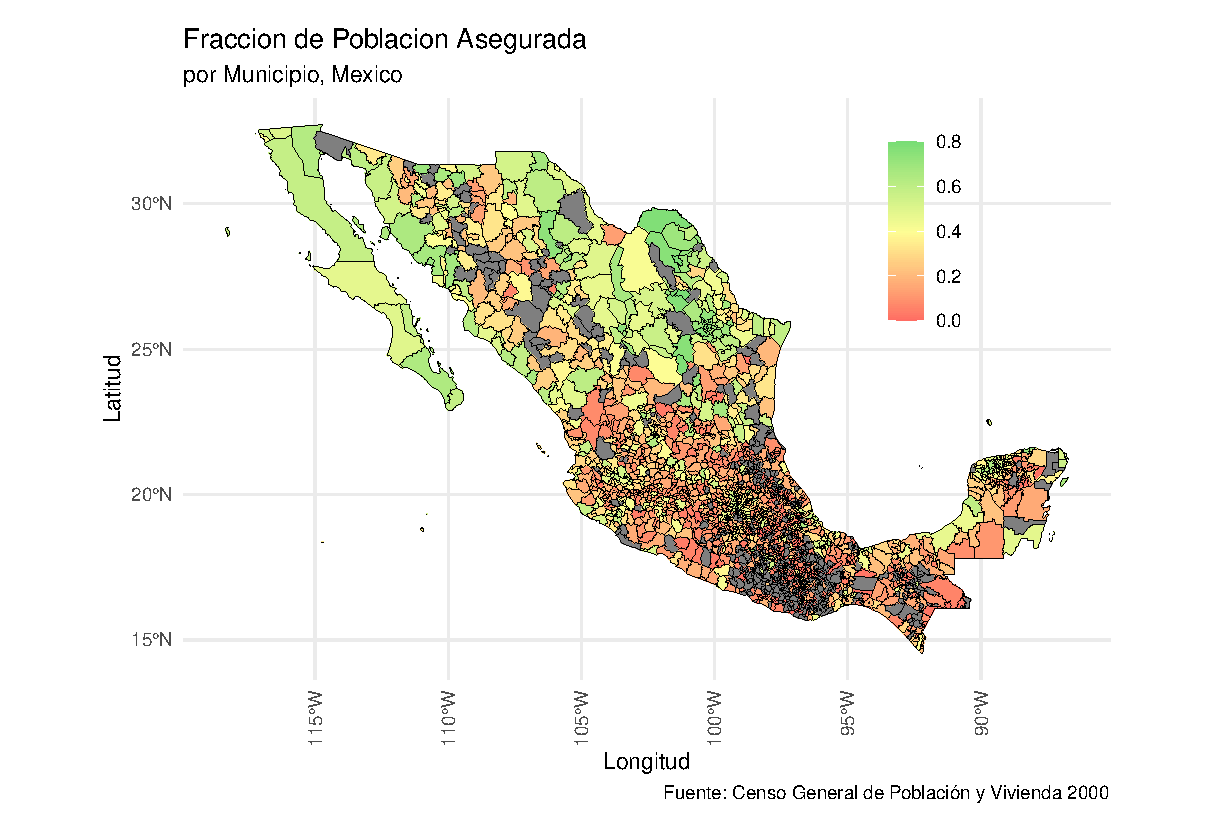
\includegraphics[width=\textwidth]{figs/insured.eps}
 \end{figure}

 A continuaci\'on se presenta la distribuci\'on de asegurados.
 \begin{figure}[H]
     \centering
     
\includegraphics[width=0.8\textwidth]{figs/histinsured.eps}
 \end{figure}
\newpage
Se presenta el siguiente un mapa con la tasa de desempleo al a\~no 2000 por municipio. Vale aclarar que solo graficamos aquellos que tengan menos de 4\% de desempleo, siendo este el 98\% de nuestra muestra.

 \begin{figure}[H]
     \centering
     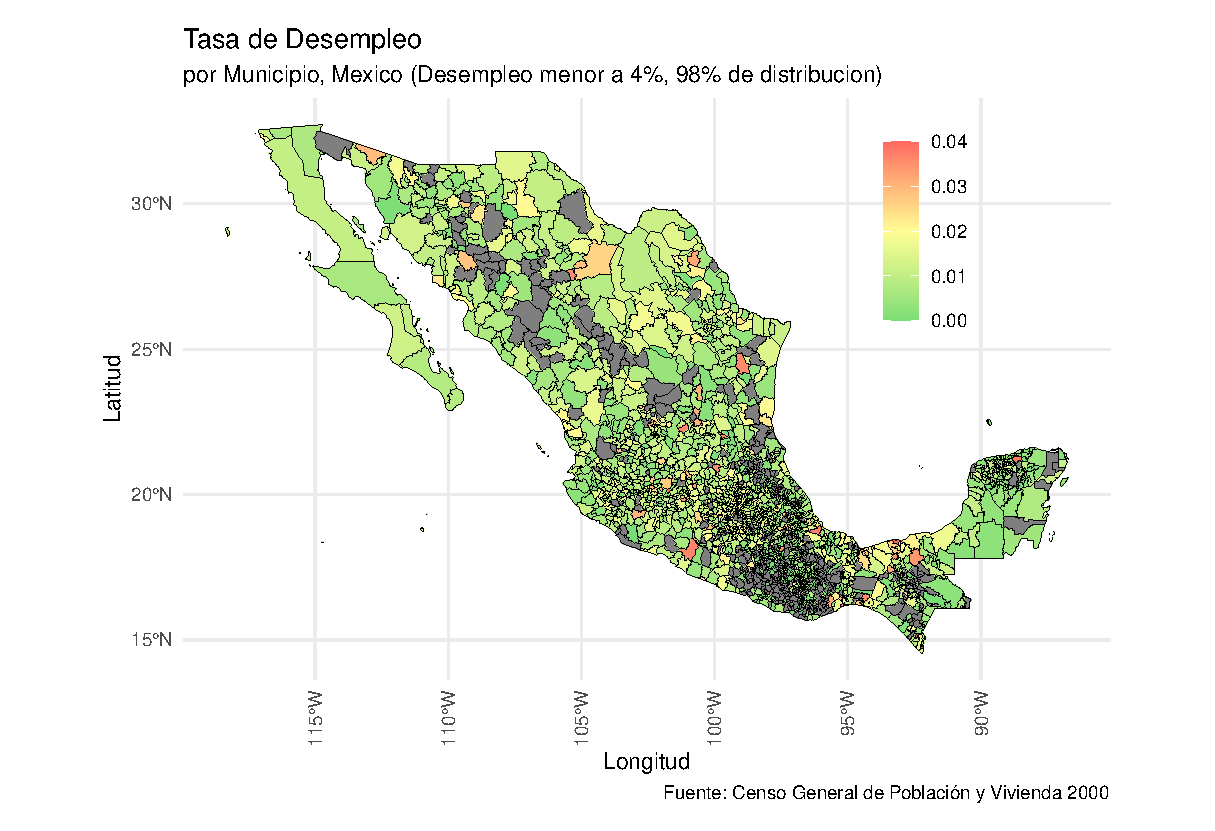
\includegraphics[width=\textwidth]{figs/unemployement.eps}
 \end{figure}
\newpage
\section*{Beneficiarios}
Con el fin de aprovechar las caracter\'isticas de la base de datos, en conjunto con este archivo se entrega un \textbf{GIF} cuya escala es en funci\'on de la cantidad de adheridos al Seguro Popular. Muestra como van entrando y saliendo municipios del programa, considerando que esta adherido al programa un municipio si en el trimestre y a\~no en cuesti\'on tienen m\'as de diez individuos. 


Sumado a esto, los autores comentan que sistemáticamente los municipios más poblados y aquellos en estados más pequeños (solo en los municipios del panel) se unieron al programa en etapas más tempranas. Para ver esto gr\'aficamente, presentamos el siguiente scatterplot entre poblaci\'on y fecha de entrada. Para definir la fecha de entrada, trabajamos con los datos para obtener la primer fecha en la cual un municipio tuvo m\'as de diez individuos adheridos al Seguro Popular. Graficamos tambi\'en la recta de regresi\'on entre ambas e incluimos el coeficiente estimado. 

\begin{figure}[H]
    \centering
    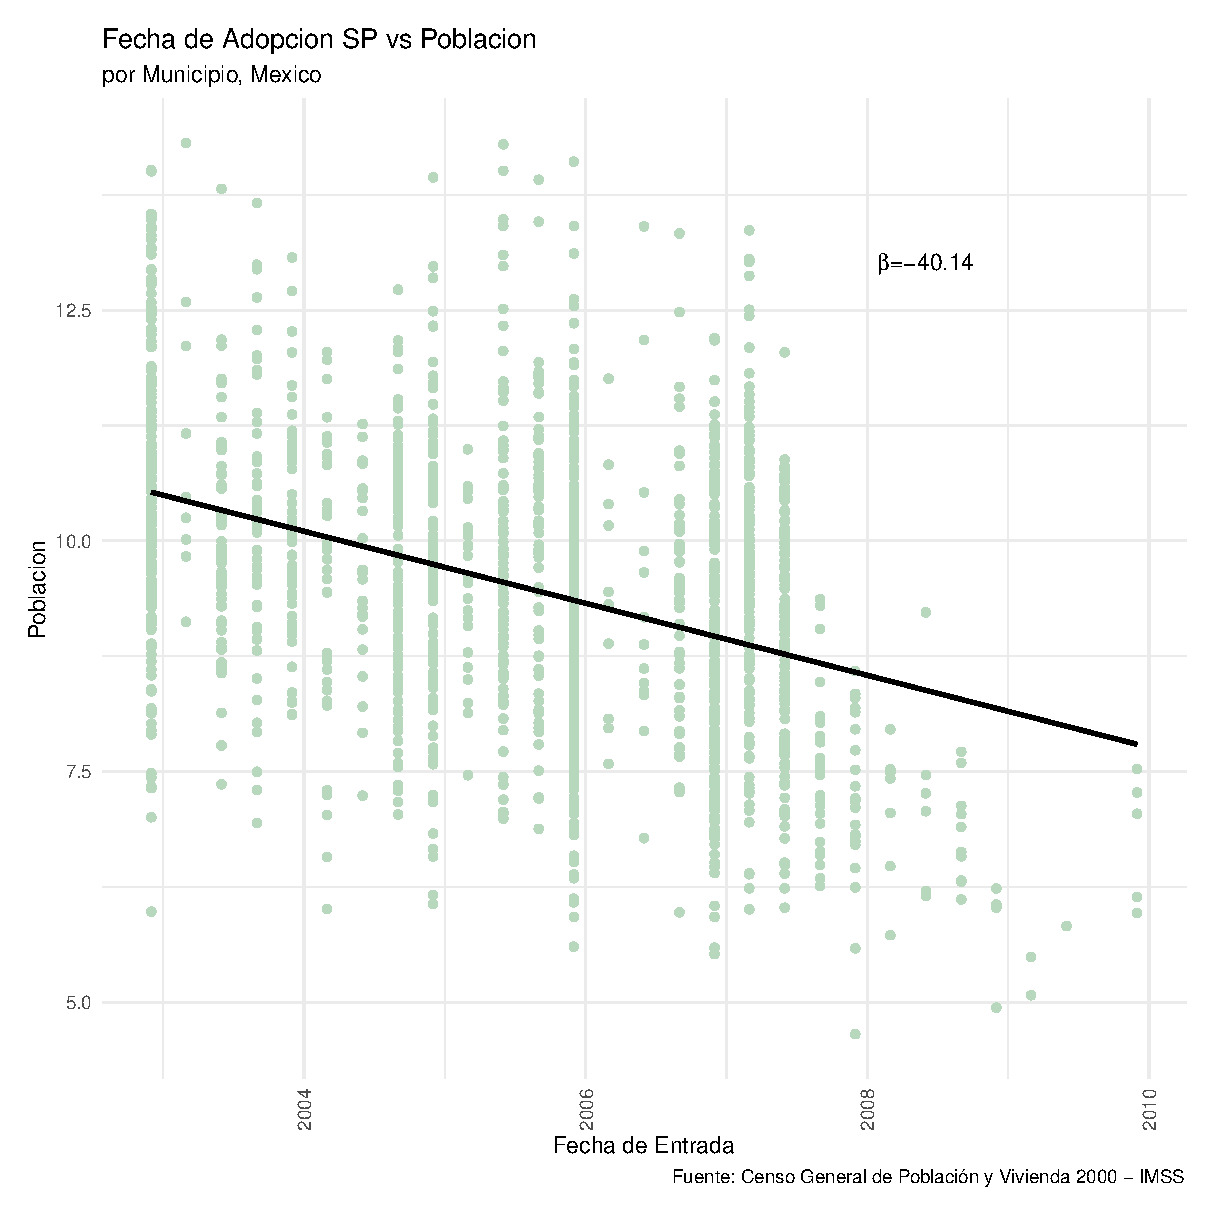
\includegraphics[width=\textwidth]{Correlacion Cami.eps}
\end{figure}
\newpage
 \section*{Empleados y Empleadores}
 De utilizar los datos de cantidad de empleadores y empleados registrados formalmente por municipio, se generaron las siguientes tablas para ver la distribuci\'on para cada a\~no de ambos grupos entre firmas de distintos tama\~nos. Se considera para cada a\~no solamente el \'ultimo trimestre. 
 
 En el caso de empleados:
 % latex table generated in R 4.1.2 by xtable 1.8-4 package
% Sun Aug 28 11:44:10 2022
\begin{table}[H]
\centering
\caption{Porcentaje de Empleados en firmas por tamaño y año (cuarto trimestre).} 
\begin{tabular}{rcccccccc}
  \toprule
  &\multicolumn{7}{c}{Cantidad de Empleados}\\ \cline{2-8}
  A\~no & 1  & 2 a 5  & 6 a 50  & 51 a 250  & 251 a 500  & 501 a 1000  & Mas de 1000  \\ 
  \midrule 2000 & 1.80 & 7.70 & 24.30 & 22.10 & 10.40 & 10.00 & 23.10 \\ 
  2001 & 1.90 & 8.20 & 25.20 & 22.60 & 10.30 & 10.00 & 21.40 \\ 
  2002 & 1.90 & 8.30 & 25.00 & 22.50 & 10.40 & 10.10 & 21.40 \\ 
  2003 & 1.90 & 8.20 & 24.80 & 22.80 & 10.60 & 10.00 & 21.20 \\ 
  2004 & 1.80 & 7.80 & 24.30 & 23.00 & 10.70 & 10.40 & 21.60 \\ 
  2005 & 1.80 & 7.50 & 23.90 & 23.40 & 10.70 & 10.30 & 22.00 \\ 
  2006 & 1.70 & 7.20 & 23.60 & 23.60 & 11.00 & 10.40 & 22.10 \\ 
  2007 & 1.70 & 7.00 & 23.40 & 23.70 & 11.00 & 10.60 & 22.30 \\ 
  2008 & 1.70 & 6.90 & 23.60 & 24.10 & 11.30 & 10.50 & 21.50 \\ 
   2009 & 1.70 & 6.90 & 23.80 & 24.50 & 11.20 & 10.40 & 21.00 \\ 
   2010 & 1.60 & 6.60 & 23.10 & 24.40 & 11.40 & 10.80 & 21.90 \\ 
   2011 & 1.50 & 6.40 & 22.70 & 24.30 & 11.50 & 10.70 & 22.70 \\ 
   \bottomrule
\end{tabular}
\end{table}


  En el caso de empleadores:
 % latex table generated in R 4.1.2 by xtable 1.8-4 package
% Sun Aug 28 11:33:22 2022
\begin{table}[ht]
\centering
\begin{tabular}{rrrrrrrrr}
  \hline
 & year & 1 Empleado & 2 a 5 Empleados & 6 a 50 Empleados & 51 a 250 Empleados & 251 a 500 Empleados & 501 a 1000 Empleados & Mas de 1000 Empleados \\ 
  \hline
1 & 2000 & 28.60 & 41.10 & 26.10 & 3.40 & 0.50 & 0.20 & 0.10 \\ 
  2 & 2001 & 28.80 & 41.30 & 25.80 & 3.30 & 0.40 & 0.20 & 0.10 \\ 
  3 & 2002 & 28.60 & 41.70 & 25.60 & 3.30 & 0.40 & 0.20 & 0.10 \\ 
  4 & 2003 & 28.60 & 41.70 & 25.60 & 3.30 & 0.50 & 0.20 & 0.10 \\ 
  5 & 2004 & 28.60 & 41.20 & 25.80 & 3.50 & 0.50 & 0.20 & 0.10 \\ 
  6 & 2005 & 28.80 & 40.60 & 26.00 & 3.70 & 0.50 & 0.20 & 0.10 \\ 
  7 & 2006 & 28.80 & 40.10 & 26.40 & 3.80 & 0.50 & 0.30 & 0.10 \\ 
  8 & 2007 & 28.80 & 39.60 & 26.80 & 3.90 & 0.50 & 0.30 & 0.20 \\ 
  9 & 2008 & 29.00 & 39.30 & 26.90 & 3.90 & 0.60 & 0.30 & 0.10 \\ 
  10 & 2009 & 29.20 & 39.00 & 26.90 & 4.00 & 0.60 & 0.30 & 0.10 \\ 
  11 & 2010 & 28.60 & 38.90 & 27.30 & 4.10 & 0.60 & 0.30 & 0.20 \\ 
   \hline
\end{tabular}
\caption{Porcentaje de Empleadores en firmas por tama�o y a�o (cuarto trimestre).} 
\end{table}


 

 \newpage
Adicionalmente, los autores resaltan que el efecto negativo en la formalidad se concentra en las firmas pequeñas y medianas, es decir, las que tienen hasta 50 empleados. De este modo, graficamos la serie de tiempo de empleadores y empleados en firmas peque\~nas y mediana como proporci\'on de empleadores y empleados totales. De considerar 2003 el a\~no que se empieza a implementar el programa\footnote{Antes era piloto.}, podemos ver que la serie va acorde a los resultados enunciados por los autores.  
\begin{figure}[H]
    \centering
    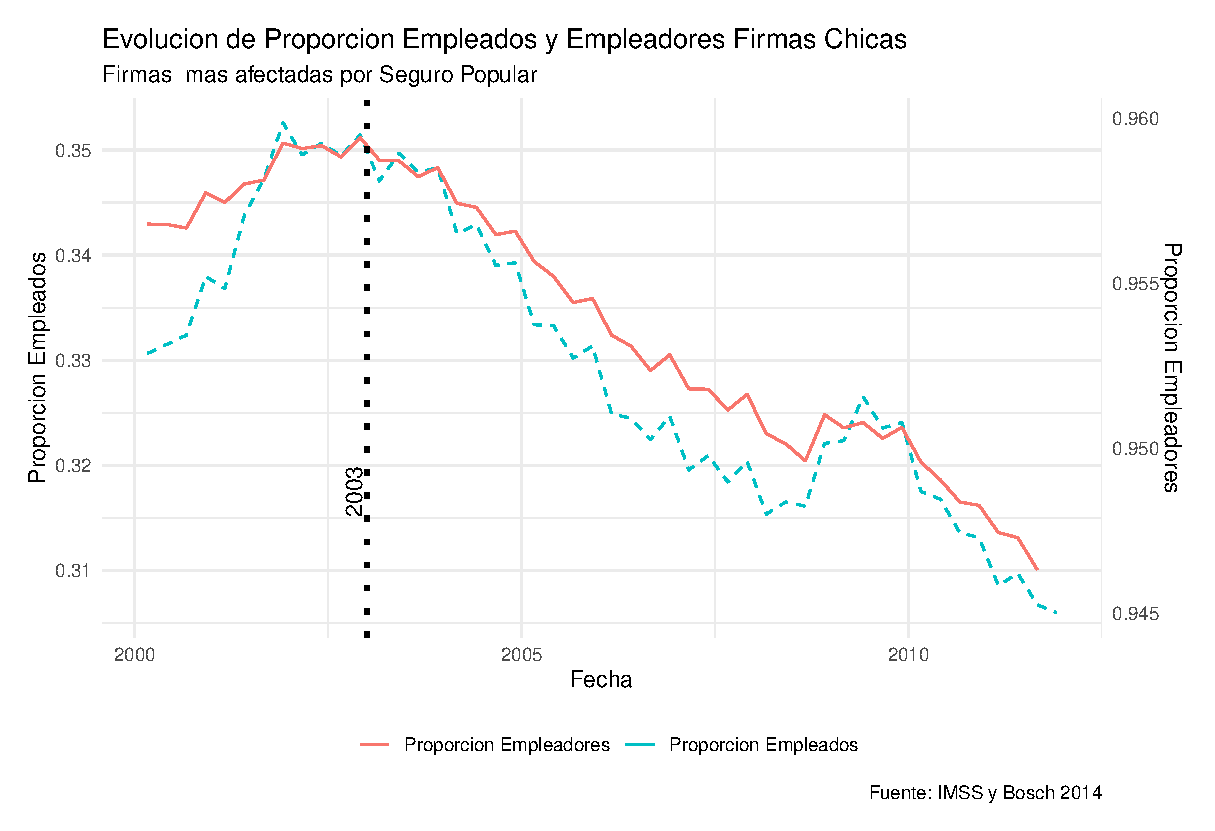
\includegraphics[width=\textwidth]{figs/smallfirms.eps}
\end{figure}

\newpage
Luego, se generan los siguientes mapas de empleados y empleadores sobre la poblaci\'on enunciada en el censo del 2000. De todos modos, estos mapas presentan ciertas inconsistencias. Hay algnos municipios donde el c\'aclculo resulta mayor a 1, as\'i como otros donde resultan muy bajos, dando indicios de que no es la mejor decisi\'on utilizar solamente datos de poblaci\'on del 2000.
 \begin{figure}[H]
     \centering
     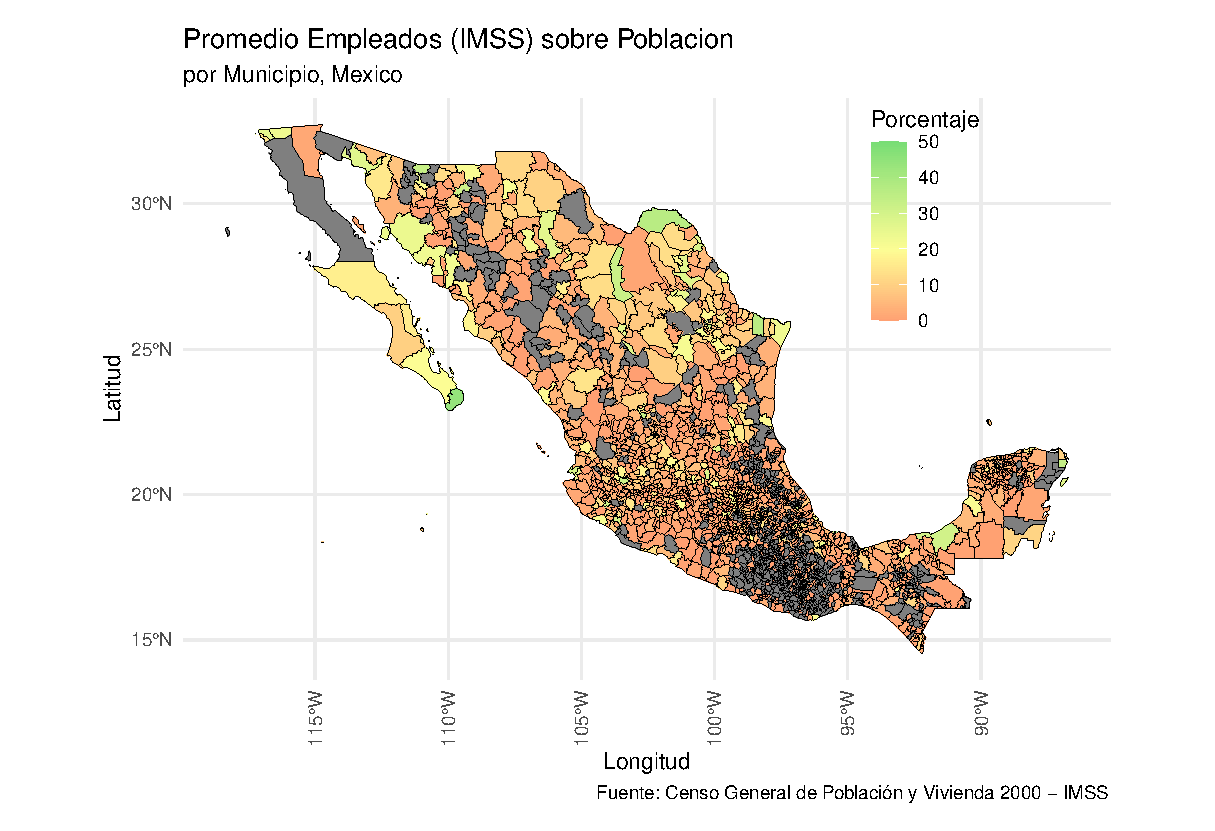
\includegraphics[width=\textwidth]{figs/employeespob.eps}
 \end{figure}
  \begin{figure}[H]
     \centering
     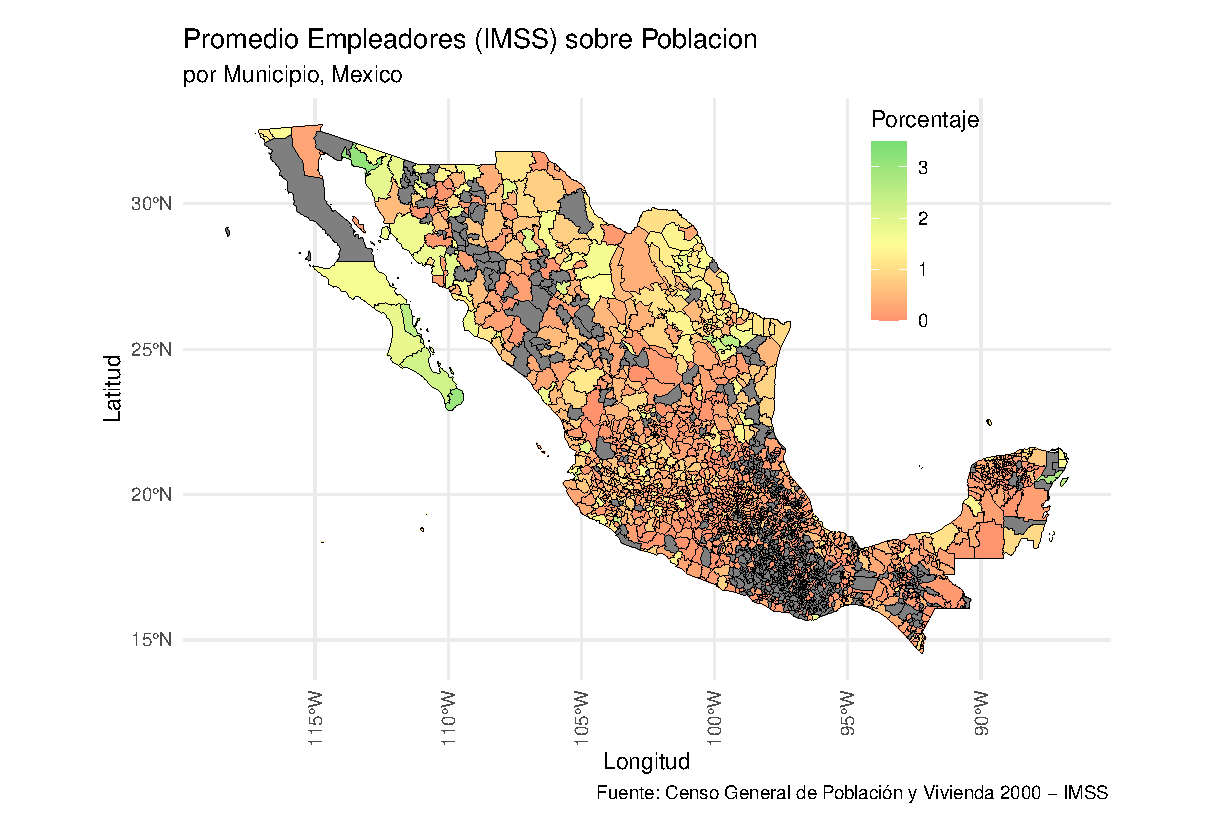
\includegraphics[width=\textwidth]{figs/employerspob.eps}
 \end{figure}
\printbibliography \end{document}

